\documentclass{kuisthesis}			% 特別研究報告書
\usepackage{listings,jlisting}
\usepackage{fancybox,ascmac}
\usepackage{amsmath}
\usepackage{tabularx}
\usepackage[dvipdfmx]{graphicx}
\usepackage{here}


\lstset{%listings の表示設定
breaklines = true,
tabsize = 2,
frame=single,
basicstyle = \small,
numbers=left,
framexleftmargin=8mm,
captionpos=b,
numberstyle=\scriptsize,
stepnumber=1,
language = Java}


\def\LATEX{{\rm (L\kern-.36em\raise.3ex\hbox{\sc a})\TeX}}
\def\LATex{\iLATEX\small}
\def\iLATEX#1{L\kern-.36em\raise.3ex\hbox{#1\bf A}\kern-.15em
    T\kern-.1667em\lower.7ex\hbox{E}\kern-.125emX}
\def\LATEXe{\ifx\LaTeXe\undefined \LaTeX 2e\else\LaTeXe\fi}
\def\LATExe{\ifx\LaTeXe\undefined \iLATEX\scriptsize 2e\else\LaTeXe\fi}
\let\EM\bf
\def\|{\verb|}
\def\<{\(\langle\)}
\def\>{\(\rangle\)}
\def\CS#1{{\tt\string#1}}

\jtitle[ IoT環境における状況依存型サービス連携の実現]%	% 和文題目(内容梗概/目次用)
	{ IoT環境における状況依存型サービス連携の実現}	% 和文題目
\etitle{Realization of situated service composition in IoT environment}	% 英文題目
\jauthor{渡辺 隆弘}				% 和文著者名
\eauthor{Takahiro Watanabe}			% 英文著者名
\supervisor{石田 亨 教授}			% 指導教員名
\date{平成28年2月6日}				% 提出年月日
\department{社会情報学}				% 修士論文の場合の専攻名

\begin{document}
\maketitle					% 「とびら」の出力

\begin{jabstract}				% 和文梗概
近年,「いつでも,どこでも,何でも,誰でも」ネットワークに繋がる「ユビキタスネットワーク社会」が構想されてきた.様々なデバイスがネットワークに接続されるようになると,それらのデバイス間での情報交換やデータの収集,それに基づく自動化が行われ,新たな付加価値を生むようになる.しかし,現状ではセンサーはただ値を取得するだけにとどまっており,ユーザのニーズにあったデータの取得というものは行うことができない.そこで,センサーデータを用いてより複雑な処理を行うために,複合サービスとの連携を行うことを考える.センサーデータを用いて複合サービスの実行を行うことで,センサーから取得できる周囲の状況に基づいて複合サービス内のサービスを選択し,複雑な処理を実行することができる.しかし,現状では,センサーに統一された枠組みが存在せず,センサーを利用するためにはそれぞれのセンサーの仕様に基づいて別々のシステムを構築する必要がある.また,IoT環境では,実環境のデータを利用するため,ユーザはリアルタイム性を求めるが,現在はデータをデータベースに格納し,抽出するため,リアルタイム性は実現できていない.\\
本研究の目的はIoT環境において状況に基づいたサービス実行を行う手法の提案と実装である.そのために,以下の2点の解決すべき課題が存在する.
\begin{enumerate}
\item センサーのサービス化\\
IoT環境では周囲のセンサーから取得されるデータや,Webから取得されるデータなど様々なフォーマットを持つデータが利用されることが考えられるため,それらの仕様の違いを気にすることなくシステムを実装できるような,統一化された枠組みを構築する必要がある.
\item リアルタイム性を保証したサービス選択\\
現在はWebサービスの選択にユーザの知識や経験が必要になる.また,ユーザはリアルタイム性を要求するため,実行するサービス選択をユーザの手を介さず,またリアルタイムに行えるようにする必要がある.
\end{enumerate}
上記の課題を解決するために,本研究では,センサーのサービス化手法を提案し,センサーデータに統一化された枠組みを与える.これにより,センサーデータを利用するシステムを実装する際,センサーの種類を考えることなく実装を行うことができる.\\
次に,センサーデータによるリアルタイムなサービス選択手法を提案する.イベント処理システムを応用し,センサーからデータを取得した際に,事前に用意したルールに従って処理を行い,利用するサービスの選択と,サービスへの入力を複合サービスに与える.この手法により,ユーザが複合サービスを利用する際に原子サービスの選択をする必要がなくなり,ユーザの知識や経験を問わず,最適なサービス選択を行うことができる.また,イベント処理システムを利用することで,センサーデータを受け取ったと同時にサービスを実行することができ,サービスのリアルタイム性も保証できる.\\
最後に,これらの提案に基づくシステムを実装した.温度,湿度センサーの存在する環境下で,センサーデータによる複合サービスのサービス選択,実行を実現した.\\
本研究の貢献は以下の2点である.
\begin{enumerate}
\item センサーのサービス化手法の提案と実装\\
センサーデータについて画一化されたデータ定義を与えることでセンサーをサービス化する手法を提案した.これにより,ユーザはセンサーの仕様を気にすることなくデータを利用することができるようになる.また,実際にセンサーサービスインターフェースを実装することで,画一された枠組みとして機能することの実例を示した.
\item リアルタイム性を保証した複合サービスのサービス選択手法の提案と実装\\
センサーの値をイベントとしてCEPエンジンに挿入し,リアルタイムで処理,アクションとして複合サービスへの入力生成とサービス実行を行うことによって,ユーザがサービスのリクエストを送信することなく,リアルタイムかつ自動的なサービス実行が可能となった.実際にこの手法を用いたシステムを実装することにより実例を示した.
\end{enumerate}
\end{jabstract}
\begin{eabstract}				% 英文梗概
In recent years, a "ubiquitous network society" connected to a network "anytime, anywhere, whatever, anyone" has been conceived. When various devices are connected to the network, information exchange between these devices, collection of data and automation based thereon are performed, and new added value is generated. However, at present, the sensor only acquires the value, and it is impossible to acquire the data that meets the needs of the user. Therefore, in order to perform more complicated processing using sensor data, consider cooperating with compound service. By executing the composite service using the sensor data, it is possible to select a service in the composite service based on surrounding situations obtainable from the sensor, and to execute complicated processing. However, at present, there is no unified framework in the sensor, and in order to use the sensor, it is necessary to construct a separate system based on the specification of each sensor. In the IoT environment, since the data of the real environment is used, the user desires real time property, but since the data is currently stored in the database and extracted, the real time property can not be realized.\\
The purpose of this research is the proposal and implementation of a method to execute service based on situation in IoT environment. Therefore, the following two problems exist.
\begin{enumerate}
\item Construct of sensor service\\
In the IoT environment, it is conceivable that data having various formats such as data acquired from surrounding sensors and data acquired from the Web are used, so that It is necessary to construct a unified framework being able to implemented the system without worrying about the difference between those specifications that can be done.
\item Service selection guaranteeing real time property\\
Currently it requires user's knowledge and experience to select web service. In addition, since the user demands real-time nature, it is necessary to select a service to be executed without intervention of the user and in real time.
\end{enumerate}
In order to solve the above problem, this research proposes a service method of sensor and gives a unified framework to sensor data. As a result, when implementing a system that uses sensor data, it is possible to implement without considering the type of sensor.\\
Next, we propose a real-time service selection method based on sensor data. By applying the event processing system, when acquiring data from the sensor, process according to the prepared rules, select the service to use and give input to the service to the composite service. This method eliminates the need for the user to select an atomic service when using a compound service and can select an optimum service regardless of user's knowledge or experience. In addition, by using the event processing system, it is possible to execute the service at the same time that the sensor data is received, and it is also possible to guarantee real-time service of the service.\\
Finally, we implemented a system based on these proposals. In the environment where temperature and humidity sensor exist, we realized service selection and execution of composite service by sensor data.\\
The contribution of this research is the following two points.
\begin{enumerate}
\item Propose and implement of method of constructing sensor service\\
We proposed a method to construct sensor service by providing unified data definition about sensor data. This allows the user to use the data without worrying about the specification of the sensor. Also, I showed an example of functioning as a standardized framework by actually installing a sensor service interface.
\item Propose and implement of service selection method of composite service with guaranteed real time property\\
By inserting the value of the sensor as an event into the CEP engine, processing in real time, input generation to the composite service and execution of the service are performed as actions, so that the user can perform automatic service execution in real time It became possible. An actual example was shown by actually implementing a system using this method.
\end{enumerate}
\end{eabstract}

\tableofcontents				% 目次の出力

\section{はじめに}\label{sec-intro}		% 本文の開始
近年,「いつでも,どこでも,何でも,誰でも」ネットワークに繋がる「ユビキタスネットワーク社会」が構想されてきた.接続機器として代表的なものとして,従来はパソコンやスマートフォンが挙げられるが,センサーデバイスの普及に伴い,車や家電といった物理機器,建物もネットワークに接続されるようになった.このように様々なデバイスがネットワークに接続されるようになると,それらのデバイス間での情報交換やデータの収集,それに基づく自動化が行われ,新たな付加価値を生むようになる.
例えば,以下のような例が挙げられる.
\begin{itemize}
\item 離れた場所の環境を知る
温度,湿度,気圧.照度といった環境をセンサーによって知ることができる.
\item 物体の動きを知る
物体の動き(衝撃,振動,移動など)を知ることができる.
\item 物体の位置を知る
物体の位置(存在,通過など)を知ることができる.
\item 機器の制御を行う
空調の制御,照明の制御などを離れた場所から操作することができる.
\end{itemize}
このような仕組みはInternet of Things(IoT)と呼ばれる仕組みであり,急速に発展している.\cite{Atzori2010}\cite{Gubbi2013}\\
また,Internet of Service(IoS)と呼ばれる,Webアプリケーションやサービスを組み合わせ,新たなサービスを構成する仕組みが存在する.\cite{Vermesan2009}

%IoTだけだと?
%IoSとIoTをつなげる必要性についての議論
本研究では,IoT環境での状況依存型サービス連携を実現することを目的とする.この目的を実現するために以下の問題点が存在する.
\begin{enumerate}
\item センサーの仕様の不統一性\\
現状は同じ種類のセンサー(温度センサーや湿度センサーなど)でも,通信手段やデータフォーマットなどに差異がある.IoT環境において,センサーデータを利用してWebサービスを実行することを考える.周囲の環境に存在するセンサーから値を取得しサービスを実行するが,そのセンサーの仕様が統一されていないために,それぞれのセンサーの仕様ごとにシステムの実装を行う必要がある.
\item リアルタイム性を保証したサービス選択\\
リアルタイム性を保証したサービス選択として,
\begin{itemize}
\item サービス選択
\item リアルタイム性
\end{itemize}
の2点について問題がある.\\
これまで,複合サービス内の原子サービスの選択は,ユーザによって指定する方向で行われてきた.例えば,言語グリッドの翻訳サービスのうち,辞書翻訳を利用することを考える.言語グリッドの辞書翻訳には様々なサービスが登録されており,ユーザがどの辞書を用いるか指定する.\\
つまり,原子サービスの選択にユーザの知識や経験が要求されるため,問題点としては以下の二つが例として考えられる.
\begin{itemize}
\item ユーザが初めて複合サービスを利用する際にどのような原子サービスを利用すれば適当かが分からない
\item ユーザのサービスに対しての知識が不足しているために,ユーザのサービス選択がユーザの要求に関わらず固定化されてしまい,ユーザの要求を満たすよりよい原子サービスの組み合わせがあるにもかかわらず,より質の低いサービス選択を行ってしまう
\end{itemize}
また,リアルタイム性については,IoT環境では,周囲の環境のデータを利用するという特性上,リアルタイムに変化する周囲の状況をその都度サービス実行に反映させることができるようにする必要があるために生じる問題である.複合サービスは,複数のWebサービスを組み合わせたものであるため,実行の仕様はWebサービスに基づく.Webサービスはリクエストに応じてレスポンスを返す形式であるため,Webサービスを利用するためには,ユーザはWebサービスにリクエストを送信する必要がある.また,現在のIoT環境では,収集したデータをデータベースに格納し,そこからデータを抽出するという形式であるために,リアルタイム性は確保されていない.
\end{enumerate}
以上の問題点があげられる.\\
本研究では,センサーのサービス化手法を提案し,センサーデータに統一化された枠組みを与える.これにより,センサーデータを利用するシステムを実装する際,センサーの種類を考えることなく実装を行うことができる.\\
次に,リアルタイム性を保証したサービス実行問題を解決するために,センサーデータによるサービス選択手法を提案する.イベント処理システムを応用し,センサーからデータを取得した際に,事前に用意したルールに従って処理を行い,利用するサービスの選択と,サービスへの入力を複合サービスに与える.この手法により,ユーザが複合サービスを利用する際に原子サービスの選択をする必要がなくなり,ユーザの知識や経験を問わず,最適なサービス選択を行うことができる.また,イベント処理システムを利用することで,センサーデータを受け取ったと同時にサービスを実行することができ,ユーザの手を介さないサービスのリアルタイム実行も実現できる.\\
最後に,これらの提案に基づくシステムを実装した.温度,湿度センサーの存在する環境下で,センサーデータによる複合サービスのサービス選択,実行を実現したものである.\\
本稿の構成は以下である.2 章では,IoTとIoSの連携に関する先行研究について記述する.3 章では ,解決すべき課題点について述べた後,提案手法としてセンサーのサービス化手法と状況依存型サービス選択手法について述べる.4 章では,3章で提案した手法を一般的なシステムに応用する際のアーキテクチャの概要について述べる.5 章では,4章で提案したアーキテクチャを用いて実装したシステムの概要,仕様について述べたのち,動作確認とシステムについての考察を行う.

\section{関連研究}\label{sec-structure}
本研究はIoT環境において周囲の状況をリアルタイムに取得し,適切なサービス連携を行うことを目的とする.
本章ではIoTについての導入と,状況依存型処理の重要性,サービス連携に関しての説明を行う.
%IoTとIoSを連携するための既存手法
%状況依存型処理のために
%イベント処理
%IoS,IoTといった単語を使わない

\subsection{Internet of Things}\label{subsec-abstract}
Internet of Things(IoT)とは,様々な物理機器,建物,乗り物などにセンサーやソフトウェアを組み込むことで,情報交換やデータの収集を行えるネットワークを構築する仕組みである.\cite{Vermesan2009}では,アイデンティティ,物理的属性,および仮想パーソナリティ,知的インターフェースを使用し、情報ネットワークにシームレスに統合されている物理的,もしくは仮想的な”モノ”に存在する標準および相互運用可能な通信プロトコルに基づく,自己構成能力を備えた動的なグローバルネットワークインフラストラクチャとして定義されている.\\
IoTは、物理的な世界と仮想的な世界を橋渡しすることで,スマートな都市,スマートな工場,資源管理、交通機関、健康、福利厚生など、多くのアプリケーション分野に影響を与える.しかし、ソフトウェアアプリケーションの中でIoTを活用することは、ネットワーキングからアプリケーション層まで,特に超大規模,極端な異質性,IoTの動的性などの大きな課題を抱えていることが指摘されている.\cite{Bouloukakis2016}
また,世界中において配備されているセンサーの数は急速に増加しており,これらのセンサーは膨大な量のデータを生成しつづけるが,それらのセンサーデータに価値を生み出すためにそれらを理解する必要がある.\cite{Perera2014}では,IoTパラダイムにおける,状況認識の重要性を明らかにしており,流動的にデータが生産しつづけられる状況下において,状況に応じた処理を行うことの必要性が示されている.

\subsection{Complex Event Processing}
Complex Event Processing(CEP,または複合イベント処理)とは,刻々と生成されるデータをリアルタイムに処理するための方式である.事前に定義したルールに,リアルタイムにデータを挿入し,そのルールに応じて即座に処理を行う.これまでのビッグデータ分析の方法は,データをデータベースに蓄積し,任意のタイミングで参照し,分析するという手法であったために,情報の処理に時間がかかるという問題点があった.CEPは対象のデータを直近の範囲に絞り,メモリ上に読みこんで処理を行うため処理を高速化でき,”直近の数秒以内に”などの条件に沿ってデータを処理することが可能となる.本研究では,このCEPをストリーム形式であるセンサーデータに対し応用することを考える.

\subsection{サービス連携}
サービス連携とは,Internet of Service(IoS)基盤に集積された各原子サービスを組み合わせ,ユーザの要求を満たす高い品質(QoS,またはQuality of Service)の複合サービス(Composite Service)を構成する技術である.Webサービスは、異なるQoSにもかかわらず,重複または同一の機能を提供するため.特定の複合サービスに参加するサービスを決定する選択肢が必要となる.\cite{Zeng2004}サービス連携の手法としては,サービス連携をQoSの最適化問題とみなして扱う研究\cite{Alrifai2009}\cite{Alrifai2010},ユーザを中心にQoSを計算する研究\cite{Lin2012}\cite{Shi2012}などがある.ユーザに対してどのようにサービスを組み合わせるかということが課題となっている.

\subsubsection{言語グリッド}
言語グリッド\footnote{http://langrid.org/jp/}\cite{Langrid}は機械翻訳などの言語資源を共有可能にする多言語サービス基盤である.多言語コミュニケーションに対する需要の高まりに比例して言語資源は急速に増加しているが,知的保護の問題や機能の違いにより利用可能性に優れない.その問題に対して,言語グリッドは,言語資源を共通のWebサービスの形式にサービス化する多言語基盤を実現することで解決している.\cite{Ishida2012a}これにより,利用者は言語グリッドにアクセスすることで,大学や研究機関,企業が提供する言語サービスを利用し,さらにそれらのサービスを組み合わせて用いることができる.また,利用者がその目的に合わせて,新たな言語サービスを作成し登録することも可能である.本研究で実装したシステムのうち,複合サービスの部分において言語グリッドを利用しており,その中でも,形態素解析,辞書連携翻訳,音声合成サービスを利用している.

\section{提案手法}
本章では,現状の課題を説明した後に,センサーのサービス化を行うための手法と,センサーから取得したデータによって,複合サービスのサービス選択,サービス実行を自動で行うための手法を提案する.

\subsection{課題点}
状況に応じたサービス選択を行うために,センサーから取得した情報によって複合サービスへの入力を変更することを考える.
その際に以下の課題点が生じる.
\begin{enumerate}
\item センサーの仕様の不統一性\\
現状は同じ種類のセンサー(温度センサーや湿度センサーなど)でも,通信手段やデータフォーマットなどに差異がある.Webサービスを利用する際には,その場所に存在するセンサーから値を取得しサービスを実行するが,そのセンサーの仕様が統一されていなければ,それぞれのセンサーの仕様ごとにシステムの実装を行う必要が生まれる.
\item 状況に応じたサービスの選択\\
これまで,複合サービス内の原子サービスの選択は,ユーザによって指定する方向で行われてきた.例えば,言語グリッドの翻訳サービスのうち,辞書翻訳\footnote{http://langrid.org/playground/dictionary.html}を利用することを考える.言語グリッドの辞書翻訳サービスは図\ref{fig:langrid}のようなインターフェースになっている.様々な種類の辞書が登録されており,ユーザはどの辞書を選択するかという情報と,翻訳したい文章を入力としてサービスに与える.\\

\begin{figure}
\label{fig:langrid}
 \begin{center}
  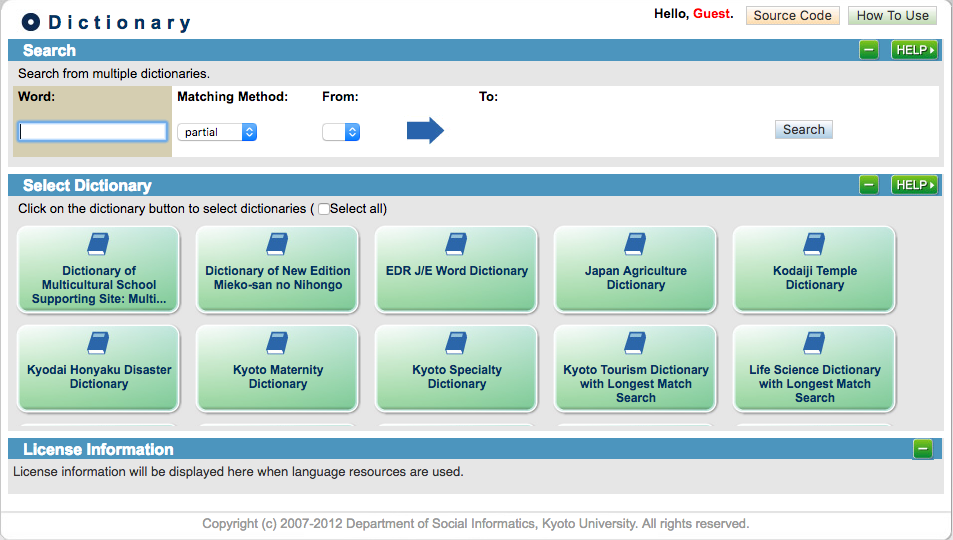
\includegraphics[width=\linewidth]{pic/langrid.png}
  \caption{言語グリッドplayground}
 \end{center}
\end{figure}


つまり,原子サービスの選択にユーザの知識や経験が要求されるため,以下のような問題点が生じる.
\begin{itemize}
\item ユーザが初めて複合サービスを利用する際にどのような原子サービスを利用すれば適当かが分からない
\item ユーザのサービスに対しての知識が不足しているために,ユーザのサービス選択がユーザの要求に関わらず固定化されてしまい,ユーザの要求を満たすよりよい原子サービスの組み合わせがあるにもかかわらず,より質の低いサービス選択を行ってしまう
\end{itemize}
\item 複合サービスのリアルタイム実行\\
複合サービスは,複数のWebサービスを組み合わせたものであるため,実行の仕様はWebサービスに基づく.Webサービスはリクエストに応じてレスポンスを返す形式であるため,Webサービスを利用するためには,ユーザはWebサービスにリクエストを送信する必要がある.
\end{enumerate}
3.2節,3.3節でこれらの課題点を解決するための手法を提案する.

\subsection{センサーのサービス化手法}
本節では,センサーのサービス化手法を提案する.現状は,前述した通りセンサーの仕様が画一化されていないために,センサーを利用するシステムを実装する際,センサーの種類によって異なる実装が必要であるという問題点が存在する.この問題点を本提案は解決する.ここで,2.3.1章に述べた言語グリッドにおける言語資源のサービス化手法を応用する.言語グリッドにおいては,複雑な契約や知的財産,データ構造やインターフェースの多様性を持つ言語資源をサービス化し共有する多言語基盤を実現している.サービスの集合知を形成する枠組みをサービスグリッドと呼び,そのためのミドルウェアが開発されている.\cite{Bus2014}\\
本研究では,言語グリッドにおける言語資源をセンサー資源に置き換える.センサー資源も言語資源と同様に,複雑なデータフォーマットやインターフェースの多様性を有している.共通のセンサーサービスインターフェースを開発することで,これらの多様性を持つセンサー資源をサービス化し,共有することが可能になる.


\begin{figure}
 \begin{center}
  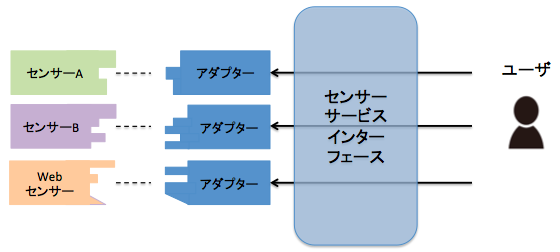
\includegraphics[width=\linewidth]{pic/sensorservice.png}
  \caption{センサーのサービス化概要}
 \end{center}
 \label{sensorservice}
\end{figure}

%言語グリッドのサービス化の話を背景にする.サービス化をどうするか
%言語資源から言語サービスへの移行 ユーザは言語グリッドが定めた標準インターフェースに基づいて実装すればよさそう これはIoT環境でもそう センサー資源からセンサーサービスへの移行
概要を図\ref{sensorservice}にしめす.現状,センサー資源はそれぞれ異なった仕様を持っている.たとえば,同じ温度を取得するものであっても,Bluetoothによる通信によってデータを送信するものや,WebセンサーとしてHTTPの形式でデータを与えるものがある.このためユーザは,それらのデータを利用しようとする際にそれぞれ異なる要求を行わなければならず,煩雑である.本提案では,センサーサービスインターフェースとしてユーザが画一化して利用できるインターフェースを設ける.センサー資源それぞれに対しアダプターという,センサー資源を画一化したインターフェースへ変換する機構を実装することでセンサーのサービス化手法として実現される.具体的にはデータ定義としてOpenIoT\footnote{http://www.openiot.eu/}のセンサー定義を用い,種々のセンサー資源から取得したデータをこのデータ形式に再形成する.OpenIoTはオープンソースで実装されているIoTプラットフォームである.OpenIoTではセンサーから取得したデータをミドルウェアを通じてデータベースに格納している.
OpenIoTのセンサー定義の例は以下のソースコード\ref{observation}であり,Observationオブジェクトとして実装される.データの値,取得時間や,温度,湿度,照度といったデータタイプを示すpropertyTypeなどが存在する.\\
\\
\begin{lstlisting}[caption=センサー定義例,label=observation]
//Observation

	private String id;	
	private Date times;	
	private String sensorId;
	private String featureOfInterest=""; 
	private ArrayList<ObservedProperty> readings;
	private String metaGraph;
	private String dataGraph;
	
	
//ObservedProperty

	private static final long serialVersionUID = 1L;
	private Object value;
	private Date times;
	private String propertyType;
	private String unit;
	private String observationId;
\end{lstlisting}

センサーの開発者は,センサーから値を取得した際に,Observationを作成し,各変数に取得した値を格納するようにサービスを構成する.システム開発者はこのサービスの仕様に従ってシステムを実装することで,ユーザからは種々のセンサー間の違いは隠蔽され,画一化されたセンサーサービスとしてデータを利用することができる.例えば,センサーから温度20℃,湿度50\%のデータを取得した際には以下のソースコード\ref{observationimpl}のようにObservationを生成する.\\
\\

\begin{lstlisting}[caption=Observation生成例,label=observationimpl]
Observation o = new Observation();    //Observationオブジェクトの作成
ArrayList<ObservedProperty> readings = new ArrayList<ObservedProperty>();     //ObservedPropertyのリストの作成
ObservedProperty tempProperty = new ObservedProperty();    //ObservedPropertyオブジェクトの作成
ObservedProperty humdProperty = new ObservedProperty();    
tempProperty.setPropertyType("http://openiot.eu/ontology/ns/AirTemperature");     //propertyTypeの設定
humdProperty.setPropertyType("http://openiot.eu/ontology/ns/AtmosphereHumidity");
tempProperty.setValue(20);    //valueに値を格納
humdProperty.setValue(50);
readings.add(tempProperty);     //ObservedPropertyのリストに追加
readings.add(humdProperty);
o.setReadings(readings);;    //Observationに作成したリストを格納
\end{lstlisting}

これにより,ユーザのリクエストは以下図\ref{service}のように簡潔化される.

\begin{figure}
 \begin{center}
  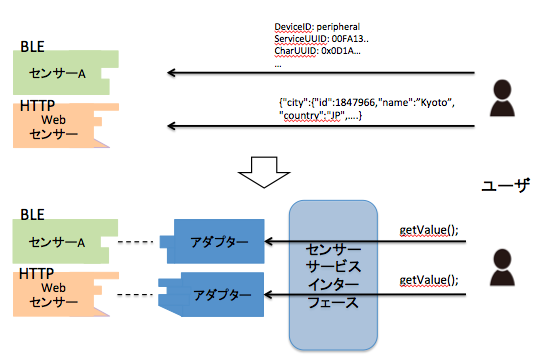
\includegraphics[width=\linewidth]{pic/service.png}
  \caption{ユーザリクエスト図}
 \end{center}
 \label{service}
\end{figure}


\subsection{状況依存型サービス選択手法}
本節では,センサーの値によって複合サービス中の原子サービスを選択する手法を提案する.センサーから取得した値をCEPエンジンによって処理することによってこの手法は実現される.まず状況によって変化させるべき部分は以下の例が存在する.
\begin{itemize}
\item 状況に応じてサービスへの入力を切り替える例
温度に応じてユーザに翻訳サービスを利用したメッセージを与えるとする.利用するサービスは翻訳サービスで変化はしないが,温度に応じてサービスへの入力を切り替える必要がある.
\item 利用するサービスを切り替える例
\item 複合サービス内の原子サービスを切り替える例
\end{itemize}

これらの状況依存型選択を行うために,ECAルールを応用することを考える.ECAルールとは,アクティブデータベースにおいて自動的に実行する処理を定義するためのルール定義であり,
\begin{description}
\item[E] : Event
\item[C] : Condition
\item[A] : Action
\end{description}
の3つからなる.イベントが発生した際,その状況に応じてアクションを実行する,というルールの実行を行う.\\
本研究では,ECAルールをCEPエンジンで実現する.つまり,ECAルールを以下のように適用する.
\begin{description}
\item[E] : センサーからのデータの取得
\item[C] : センサーから取得した値
\item[A] : 選択するサービスとサービスへの入力の生成,サービスの実行
\end{description}
以上から,センサーからデータを取得した際,サーバーからCEPエンジンにデータを挿入し,事前に定義されたルールに基づいて,選択するサービスとサービスへの入力の生成とサービスの実行を行うという一連の処理が実行される.また,本研究ではCEPエンジンにおいて適用するルールは事前に定義されているものとし,状況に応じてどのような処理を実行すべきかというルールの構成の点についての議論は行わない.\\
この手法により以下の2点の問題点が解決される.%ここを頭に

\begin{enumerate}
\item 複合サービス内の原子サービスの選択\\
ユーザがサービス選択を行わなければならないという問題点が存在した.一方,本提案では,専門家が一度ルールを作成すれば,センサーの値によって分岐するルールに従って原子サービスの選択を行うことができ,サービス連携においてユーザのサービスに対しての知識や経験に関わらず一定の質の高いサービス合成が可能となる.
\item 複合サービスのリアルタイム実行\\
サービス実行のためにユーザはWebサービスにリクエストを送信する必要があった.一方,本提案では,センサーの値をイベントとしてCEPエンジンに挿入し,リアルタイムで処理,アクションとして複合サービスへの入力生成とサービス実行を行うことによって,ユーザがサービスのリクエストを送信することなく,リアルタイムかつ自動的なサービス実行が可能となる.
\end{enumerate}

\section{提案アーキテクチャ}
本章では,前章に説明した提案手法に基づいて,IoT環境下で複合サービスの選択,実行を行うシステムのアーキテクチャの提案を行う.アーキテクチャは大きく分けてセンサーデバイス,ユーザデバイス,複合サービスの3つの領域に分割される.ユーザデバイスの内部にセンサーからのデータを受け取りサーバーへ送信するレシーバー,データを受け取り,イベントを構成してCEPエンジンに挿入するサーバー,システム開発者が規定したルールに基づいて挿入されたイベントの処理を行い,複合サービスへ入力を与えるCEPエンジンが存在する.
%要求,機能,主要なモジュール

\subsection{アーキテクチャ図}
提案するアーキテクチャのアーキテクチャ図を以下\ref{pic:archi}に示す.
\begin{figure}
 \begin{center}
  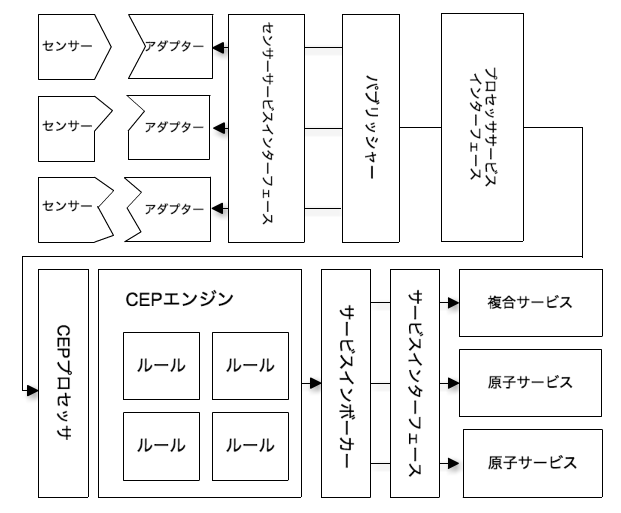
\includegraphics[width=\linewidth]{pic/Architectureimple.png}
  \caption{アーキテクチャ図}
  \label{pic:archi}
 \end{center}
\end{figure}

\subsection{センサーサービスインターフェース}
センサーサービスインターフェースは3.2節で説明したセンサーのサービス化手法を用いて,種々のセンサー間の差異を覆い隠すラッパーとしての役割を果たす.ユーザデバイスがセンサーから値を取得する際の統一された枠組みとして存在し,レシーバーに対し規定された形でデータを送信する.
\subsection{パブリッシャー}
パブリッシャーはセンサーサービスインターフェースを介してそれぞれのセンサーからデータを取得するレシーバーとしての役割と,データを処理部であるCEPプロセッサに送信する役割を持つ.パブリッシャーがデータを取得するためのリクエストは,センサーサービスインターフェースの仕様に基づき一元化されている.
\subsection{プロセッササービスインターフェース}
サーバーに挿入されたイベントを,規定されたルールに基づいて処理する.ルールはシステムの設計者が自由に定めることができ,「あるイベントが起きた際に何らかの処理が行われる」という形のECAルールで規定される.ルールエンジンはイベントの処理の結果,利用する複合サービスの仕様に基づいて入力を生成し,複合サービスへ与える.例として複合サービス内の選択サービスとサービスへの入力が挙げられる.例として,言語グリッドの場合は,
\begin{description}
\item[選択サービス] 辞書翻訳,使用する辞書
\item[入力] 翻訳元言語,翻訳先言語.翻訳したい文章
\end{description}
を言語グリッドに与えると,辞書翻訳を利用できる.イベント挿入後,イベントの処理を行うタイミングは任意であり,挿入と同時に処理を行うことでリアルタイムな複合サービスの実行が実現できる.
\subsection{CEPプロセッサ}
複合サービスは構成要素として複数の原子サービスまたは複合サービスがあり,それぞれのサービスを組み合わせて新たなサービスを実行することができる.CEPエンジンから入力が与えられたら,サービスを実行し,ユーザに出力として与える.
\section{実装}
本章では,前章に提案したアーキテクチャの実装について説明し,動作確認と評価について述べる.最後に実装の結果に対して考察を行う.


\subsection{シチュエーション}
体育館を利用するユーザに,温度,湿度などの情報から運動への助言を音声で与えるシステムを実装することを考える.ユーザは様々な言語圏のユーザが想定されるため,それぞれのユーザが利用する言語に基づいてアナウンスを行う必要がある.体育館には温度センサー,湿度センサーが存在しており,システムはそれらのセンサーから取得したデータと,ユーザが自身の使用する言語を自身の持つデバイスによりシステムに与えた入力に基づいてサービスを実行する.音声はユーザデバイスではなくシステムを含むコンピュータから出力される.

\subsection{仕様}
Javaを用いて実装した.以下に各モジュールの詳細を述べる.実装図は以下図\ref{pic:system}である.
\begin{figure}[hb]
 \begin{center}
  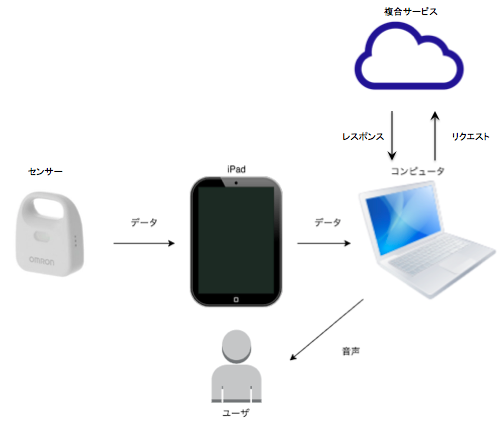
\includegraphics[width=\linewidth]{pic/system.png}
  \caption{実装概要}
  \label{pic:system}
 \end{center}
\end{figure}
大きく分けてセンサーデバイス部,ユーザデバイス部,メイン部,複合サービス部に分けられる.
%名前わけ

\subsubsection{センサーデバイス部}
体育館に設置することを想定するセンサーデバイスは,(株)オムロンの環境センサー\footnote{http://www.omron.co.jp/ecb/products/sensor/special/environmentsensor/}とする.このセンサーによって取得できるデータタイプの中から,今回は温度データと湿度データを利用する.センサーはBluetooth Low Energy(BLE)を用いて通信を行う.
\subsubsection{ユーザデバイス部}
ユーザデバイス部では,
\begin{itemize}
\item アダプター
\item パブリッシャー
\end{itemize}
の2つを備えたアプリケーションを実装した.全体として,センサーから取得したデータと,ユーザから入力された使用言語の情報を統一されたインターフェースとして形成し,メイン部に送信する役割を果たす.
構成要素は以下.
\begin{itemize}
\item アダプター\\
取得したデータをセンサーサービスインターフェースとしてOpenIoTのセンサー定義を用いてサービス化する.取得される情報は,
\begin{itemize}
\item 温度データ
\item 湿度データ
\item 利用者の言語情報
\end{itemize}
の三つである.温度データ,湿度データについては,センサーデータより値とデータタイプを取得し,Observation[\ref{observation}]中のObservationProperty[\ref{observedprop}]のうち,valueとpropertyTypeに格納する.手順は以下.
\begin{enumerate}
\item Observationオブジェクトを生成する.
\item ObservedPropertyとしてtempProperty,humdPropertyを作成する.それぞれ,温度のデータ,湿度のデータを格納するオブジェクトである
\item ObservedPropertyそれぞれに,データタイプを示すPropertyTypeとデータの値を格納する.
\item tempPropertyとhumdPropertyをObservationオブジェクトに格納する.
\end{enumerate}

\item パブリッシャー\\
パブリッシャーは生成したObservationオブジェクトをサーバに送信する.
\end{itemize}

\subsubsection{メイン部}
メイン部では
\begin{itemize}
\item プロセッササービスインターフェース
\item CEPプロセッサ
\item CEPエンジン
\item ルール
\item スピーカー
\end{itemize}
の5つを実装した.全体として,ユーザデバイスから取得したデータをルールエンジンで処理し,複合サービスへの入力を生成し,送信する役割を果たす.また,音声合成サービスにより生成された音声ファイルを再生する.
\begin{itemize}
\item CEPエンジン\\
CEPエンジンとして,Javaで実装されたイベントエンジンであるDrools\footnote{https://www.drools.org/}を利用する.DroolsはJavaで実装されたルールエンジンである.中心となるのは推論エンジンであり,事前に構成したルールに基づき,事実に対して条件が真のものを実行する.ルール言語としてDrools Rule Language(DRL)を使用する.DRLファイルは複数のルール,クエリ,型,関数,およびリソース宣言を指定するテキストファイルである.ルールはソースコード\ref{drl}のように構成される.ルールは3.3.2節で説明したECAルールに基づいており,ある条件を満たすセンサーデータが取得された際に,それに応じた処理として選択するサービスとサービスへの入力を生成し,サービスに与えるという処理が行われる.
\begin{lstlisting}[caption=drlファイル仕様,label=drl]
rule "名前"
when
    <処理を実行する際のセンサーデータの値>*
then
    <選択するサービスとサービスへの入力をサービスに与える>*
end
\end{lstlisting}
%Reteアルゴリズム?
\item ルール\\
ルールとして"badminton.drl"を実装した.ルールの概要を表\ref{tab:drl}に挙げる.本実装はWet Bulb Globe Temperature(湿球黒球温度,WBGT)を,ユーザへの注意喚起の基準として用い,今回は
\begin{equation}
WBGT = \begin{cases}
T + (H - 80)/5 & (80 \leq H) \\
T -(80 -H)/5 & (H < 80)
\end{cases}
\label{wbgt}
\end{equation}
\begin{flushright}
T:temperature(℃),H:humidity(\%)
\end{flushright}
と温度と湿度の値から近似して求める.
ルールファイルは大きく分けて5つのルールから構成されている.
%サービス選択がどうなるか
\begin{itemize}
\item WBGCClacルール\\
温度データと湿度データ,利用言語の情報が挿入された際に実行されるルールであり,ユーザデバイスからイベントが挿入された際に最初に実行されるルールである.湿度80\%を基準としてルールは分岐し,それぞれ式(\ref{wbgt})に基づいてWBGTの値を計算する.その後,求めたWBGTをvalueとし,propertyTypeとしてWBGTを持つObservedPropertyと,入力された言語をvalue,propertyTypeとしてTargetLanguageを持つObservedPropertyを追加してObservationを生成し,ルールファイルにイベントとして再挿入する.
\item Phaseルール\\
Phaseルールはユーザに周囲の温度,湿度によって運動への注意喚起を行うためのルールである.WBGCClacルールによって再挿入されたイベントにより実行されるルールであり,WBGTの値によって5つに細分化される.言語グリッドの辞書翻訳サービスと音声合成サービスにそれぞれ入力を与え,その結果をスピーカーによって出力する.
\item Shuttleルール\\
Shuttleルールは,バドミントンをするユーザが使用するべき適切なシャトルコックの種類を温度に応じて提示するルールである.温度の値によって6つに細分化される.言語グリッドの辞書翻訳サービスと音声合成サービスにそれぞれ入力を与え,その結果をスピーカーによって出力する.
\item Stringsルール\\
Stringsルールはバドミントンをするユーザのラケットのストリングスの張る強さについて助言を与えるためのルールである.温度の値によって3つに細分化される.言語グリッドの辞書翻訳サービスと音声合成サービスにそれぞれ入力を与え,その結果をスピーカーによって出力する.
\item floorルール\\
floorルールは体育館を利用するユーザに対し,湿度による体育館の床への影響について注意喚起を行うルールである.湿度が90\%以上の際に実行され,言語グリッドの辞書翻訳サービスと音声合成サービスにそれぞれ入力を与え,その結果をスピーカーによって出力する.
\end{itemize}

\begin{table}[p]
  \begin{center}
    \caption{badminton.drl}
    \begin{tabularx}{\linewidth}{|c|c|X|} \hline
      ルール名 & 条件 & 出力 \\ \hline \hline
      WBGCcalc1 & H $\geq$ 80 & WBGTの計算 WBGT $=$ T + (H - 80)/5  \\
      & & Propertytypeの作成:WBGT,Temperature \\
      & & Humidity,targetlanguageについて \\ 
      & & 再構成したObservationの再挿入 \\ \hline
      WBGCcalc2 & H $<$  80 & WBGTの計算 WBGT $=$ T - (80 - H)/5  \\
      & & Propertytypeの作成:WBGT,Temperature \\
      & & Humidity,targetlanguageについて \\ 
      & & 再構成したObservationの再挿入 \\ \hline \hline
      \multicolumn{3}{|c|}{イベントの再挿入後,テキストと利用サービスを} \\
      \multicolumn{3}{|c|}{Webサービスへの入力としたルールが実行される} \\ \hline \hline
      Phase & \multicolumn{2}{c|}{辞書翻訳(スポーツ辞書)サービスと音声合成サービスを} \\
      ルール & \multicolumn{2}{c|}{利用し,運動中のユーザへの注意喚起を行う} \\ \hline \hline
      Phase5 & WBGT $\geq$ 31  & 入力: "運動を中止しましょう."\\ \hline
      Phase4 & 28 $\leq$ WBGT $<$ 31 & 入力: "激しい運動は避け、積極的に休息と水分補給を行いましょう."\\ \hline
      Phase3 & 25 $\leq$ WBGT $<$ 28 & 入力: "激しい運動を行う際は,30分おきくらいに休息をとりましょう."\\ \hline
      Phase2 & 21 $\leq$ WBGT $<$ 25 & 入力: "水分補給には十分気をつけましょう."\\ \hline
      Phase1 & WBGT $<$ 21 & 入力: "熱中症の危険は少ないですが,適宜水分補給をしましょう."\\ \hline \hline
      Shuttle & \multicolumn{2}{c|}{辞書翻訳(バドミントン辞書)サービスと音声合成サービスを} \\
      ルール & \multicolumn{2}{c|}{利用し,シャトルコックの選択に関する情報を与える} \\ \hline \hline
      shuttle1 & T $\geq$ 33 & 入力:"1番のシャトルを使いましょう." \\ \hline 
      shuttle2 & 27 $\leq$ T $<$ 33 & 入力:"2番のシャトルを使いましょう."  \\ \hline
      shuttle3 & 22 $\leq$ T $<$ 27& 入力:"3番のシャトルを使いましょう."  \\ \hline
      shuttle4 & 17 $\leq$ T $<$ 22 & 入力:"4番のシャトルを使いましょう."  \\ \hline
      shuttle5 & 12 $\leq$ T $<$ 17 & 入力:"5番のシャトルを使いましょう."  \\ \hline
      shuttle6 & T $<$ 12 & 入力:"6番のシャトルを使いましょう." \\ \hline \hline
    \end{tabularx}
    \label{tab:drl}
  \end{center}
\end{table}

\begin{table}[htb]
    \begin{tabularx}{\linewidth}{|c|c|X|} \hline
      ルール名 & 条件 & 出力 \\ \hline \hline
      Strings & \multicolumn{2}{c|}{辞書翻訳(バドミントン辞書)サービスと音声合成サービスを} \\
      ルール & \multicolumn{2}{c|}{利用し,ラケットのストリングスに関する情報を与える} \\ \hline \hline
      strings1 & T $>$ 25 & "適正温度のときより+1ポンドのガットが適切です."  \\ \hline
      strings2 & 15 $\leq$ T $\leq$ 25 & "適正" \\ \hline
      strings3 & T $<$ 15 & "適正温度のときより-1ポンドのガットが適切です." \\ \hline
      floor & \multicolumn{2}{c|}{辞書翻訳(スポーツ辞書)サービスと音声合成サービスを} \\
      ルール & \multicolumn{2}{c|}{利用し,体育館の床面の結露による転倒を警告する} \\ \hline \hline
      floor & H $\geq$ 90 & "湿度が高く床が滑りやすくなっています.気をつけましょう." \\ \hline
    \end{tabularx}
\end{table}

\end{itemize}

\subsubsection{複合サービス部}
複合サービスとして,言語グリッドを利用する.言語グリッドは,登録された言語サービスを自由に組み合わせて新しい言語サービスを生み出すサービス連携基盤である.本研究では,言語グリッドに登録されているサービスの中から,最長一致辞書連携翻訳サービス,音声合成サービスを利用する.
%複合サービスのフレーム
\begin{itemize}
\item 翻訳部\\
翻訳部は,言語グリッドから提供されているサービスの中から,最長一致辞書連携翻訳サービスを利用する.このサービスは,形態素解析サービス,最長一致二ヶ国語辞書サービス,翻訳サービスからなる.これらの複合サービス内から提供されているサービスを自由に組み合わせることができる.本実装では,
\begin{description}
\item[形態素解析サービス] MeCab
\item[最長一致二ヶ国語辞書サービス] スポーツ辞書翻訳サービス
\item[翻訳サービス] KyotoUJServer
\end{description}
を利用する.それぞれ利用するサービスを選択し,翻訳元言語,翻訳先言語,翻訳したい文を入力として与えると,結果として,それらのサービスを利用した翻訳文を返す.
\item 音声合成部\\
音声合成部は,言語グリッドにおいて提供されている音声合成サービス(VoiceTextサービス)を利用する.入力として音声を流す言語,音声化するテキスト,オーディオファイルの形式を与えると,入力に応じたオーディオファイルを生成する.作成されたオーディオファイルを流すためのスピーカーモジュールを新たに実装することで,音声合成,出力部として実装した.\\
以上より,前5.2.3節に基づいて生成されたサービスへの入力に基づいてテキストの翻訳を行い,音声出力を行うという一連の機能が実装される.
\end{itemize}

\subsection{考察}
本節では,5.2節で実装したシステムについて考察を与える.\\
まず,本実装では,センサー資源として(株)オムロンの環境センサーと,無料天気予報APIであるOpenWeatherMap\footnote{http://openweathermap.org/}を用いた.ユーザは環境センサーはBLEによって,OpenWeatherMapはJSONによってデータを取得する.両者の仕様は大きく異なるため,データを利用する際に別々のデータ取得モジュールを実装する必要があった.本実装においては,共通のセンサーサービスインターフェースと,それと環境センサー,OpenWeatherMapをつなぐアダプターを実装することで,データ取得部を一通りの実装で実現することができた.また,ユーザの利用言語もこのインターフェースの形に形成し,利用出来ることを示した.このように,新たなセンサー資源が増えた際も,センサーの仕様に合わせてアダプターを実装すれば,それまでの既存のシステムが適用できる.\\
次に,サービス連携について,本実装では,CEPエンジンを用い,状況に合わせて利用するサービスやサービスに与える入力を自動で生成するという方法を取った.結果として,周囲の温度,湿度に応じて言語グリッドの利用サービスと入力が変化させることができることを確認した.しかし,問題点もいくつか浮上した.一つ目はサービス連携のQoSに関する課題である.サービス連携において,QoSは重要視される点であるが,本実装では経験のあるユーザ(専門家)が事前に決めたルールに基づいてサービス合成を行っているため,システムを利用するユーザそれぞれに対しQoSが最高であるサービスの組み合わせが行なわれているとは限らない.もう一つはセンサーデータの利用法である.本実装では,データを取得する度にルールを実行し,サービス実行を行っている.しかし,実際は,温度や湿度といったデータは短時間で急激に変化することは考えにくく,また,ごく近い距離同士に設置されたセンサーで取得したデータ間に大きな違いがあるとは考えにくい.センサーデータは膨大な量であるために,これらの時間的,あるいは距離的特徴を捉え,よりコストのかからないデータ取得法が必要であると考えられる.
%どういう改良ができるか




\section{終わりに}
本研究では,センサーのサービス化手法を提案し,センサーデータに統一化された枠組みを与えた,センサーデータを利用するシステムを実装する際,センサーの種類を考えることなく実装を行うことを可能とした.\\
次に,複合サービス内の原子サービスの選択問題の解決と,サービスのリアルタイム実行の2点を解決するために,センサーデータによるサービス選択手法を提案した.イベント処理システムを応用し,センサーからデータを取得した際に,事前に用意したルールに従って処理を行い,利用するサービスの選択と,サービスへの入力を複合サービスに与える.この手法により,ユーザが複合サービスを利用する際に原子サービスの選択をする必要がなくなり,ユーザの知識や経験を問わず,最適なサービス選択を行うことができた.また,イベント処理システムを利用することで,センサーデータを受け取ったと同時にサービスを実行することができ,ユーザの手を介さないサービスのリアルタイム実行も実現した.\\
最後に,これらの提案に基づくシステムを実装した.温度,湿度センサーの存在する環境下で,センサーデータによる複合サービスのサービス選択,実行を実現したものである.\\
本研究の貢献は以下の2点である.
\begin{enumerate}
\item センサーのサービス化手法の提案と実装\\
センサーデータについて画一化されたデータ定義を与えることでセンサーをサービス化する手法を提案した.これにより,ユーザはセンサーの仕様を気にすることなくデータを利用することができるようになる.また,実際にセンサーサービスインターフェースを実装することで,画一された枠組みとして機能することの実例を示した.
\item リアルタイム性を保証した複合サービスのサービス選択手法の提案と実装\\
センサーの値をイベントとしてCEPエンジンに挿入し,リアルタイムで処理,アクションとして複合サービスへの入力生成とサービス実行を行うことによって,ユーザがサービスのリクエストを送信することなく,リアルタイムかつ自動的なサービス実行が可能となった.実際にこの手法を用いたシステムを実装することにより実例を示した.
\end{enumerate}

\acknowledgments				% 謝辞
本研究を行うにあたり,貴重な資料をご提供いただきました株式会社オムロン様に深く感謝申し上げます.そして本研究を行うにあたり,熱心なご指導,ご助言を賜りました石田亨教授に厚く御礼申し上げます.また,日頃より数々のご助言をいただきました中口孝雄特定研究員,林冬惠助教をはじめ,石田・松原研究室の皆様方に心より感謝いたします.
\nocite{*}
\bibliographystyle{kuisunsrt}			% 文献スタイルの指定
\bibliography{library}

\Appendix[付録]
実装のソースコードを添付する.

\section{デバイスでセンサーデータを取得し、サーバーへ送信するモジュールのソースコード}
\subsection{MyviewController.java}
\lstinputlisting{/Users/admin/Documents/OpenIoT_integration/waikikisens/src/main/java/org/langrid/waikiki/sensor/MyviewController.java}

\subsection{WaikikiSensor.java}
\lstinputlisting{/Users/admin/Documents/OpenIoT_integration/waikikisens/src/main/java/org/langrid/waikiki/sensor/WaikikiSensor.java}

\section{受信したデータをルールエンジンに挿入し、状況に応じた出力を得るモジュールのソースコード}

\subsection{ObservationReceiverImpl.java}
\lstinputlisting{/Users/admin/Documents/OpenIoT_integration/waikikiws/src/main/java/org/langrid/waikikiws/service/ObservationReceiverImpl.java}

\subsection{Translator.java}
\lstinputlisting{/Users/admin/Documents/OpenIoT_integration/waikikiws/src/main/java/org/langrid/waikikiws/service/Translator.java}

\subsection{Binding.java}
\lstinputlisting{/Users/admin/Documents/OpenIoT_integration/waikikiws/src/main/java/org/langrid/waikikiws/Bindings.java}

\subsection{DroolsManager.java}
\lstinputlisting{/Users/admin/Documents/OpenIoT_integration/waikikiws/src/main/java/org/langrid/waikikiws/DroolsManager.java}

\subsection{DroolsUtil.java}
\lstinputlisting{/Users/admin/Documents/OpenIoT_integration/waikikiws/src/main/java/org/langrid/waikikiws/DroolsUtil.java}

\subsection{TargetLanguage}
\lstinputlisting{/Users/admin/Documents/OpenIoT_integration/waikikiws/src/main/java/org/langrid/waikikiws/service/TargetLanguage.java}

\subsection{VoiceText.java}
\lstinputlisting{/Users/admin/Documents/OpenIoT_integration/waikikiws/src/main/java/org/langrid/waikikiws/VoiceText.java}

\subsection{TransTextToSpeech.java}
\lstinputlisting{/Users/admin/Documents/OpenIoT_integration/waikikiws/src/main/java/org/langrid/waikikiws/TransTextToSpeech.java}

\subsection{badminton.drl}
\lstinputlisting{/Users/admin/Documents/OpenIoT_integration/waikikiws/src/main/resources/badminton.drl}

\section{オムロンのセンサー定義}
\subsection{EnvSensor.java}
\lstinputlisting{/Users/admin/Documents/OpenIoT_integration/waikikisens/src/main/java/org/langrid/waikiki/sensor/omron/EnvSensor.java}

\subsection{EnvSensorListener.java}
\lstinputlisting{/Users/admin/Documents/OpenIoT_integration/waikikisens/src/main/java/org/langrid/waikiki/sensor/omron/EnvSensorListener.java}

\subsection{EnvSensorScanner.java}
\lstinputlisting{/Users/admin/Documents/OpenIoT_integration/waikikisens/src/main/java/org/langrid/waikiki/sensor/omron/EnvSensorScanner.java}

\section{OpenIoTのデータ定義}
\subsection{Observation.java}
\lstinputlisting[label=observation]{/Users/admin/Documents/OpenIoT_integration/waikikiws/src/main/java/org/openiot/lsm/beans/Observation.java}

\subsection{ObserbationProperty.java}
\lstinputlisting[label=observedprop]{/Users/admin/Documents/OpenIoT_integration/waikikiws/src/main/java/org/openiot/lsm/beans/ObservedProperty.java}

\end{document}
